% Name: Planar graph and its dual
% Description: A square with one diagonal in black, and its dual in red: one vertex per face, the outer face included, and one dual edge across each edge.
% Tags: planar graph, dual graph, faces, graph theory

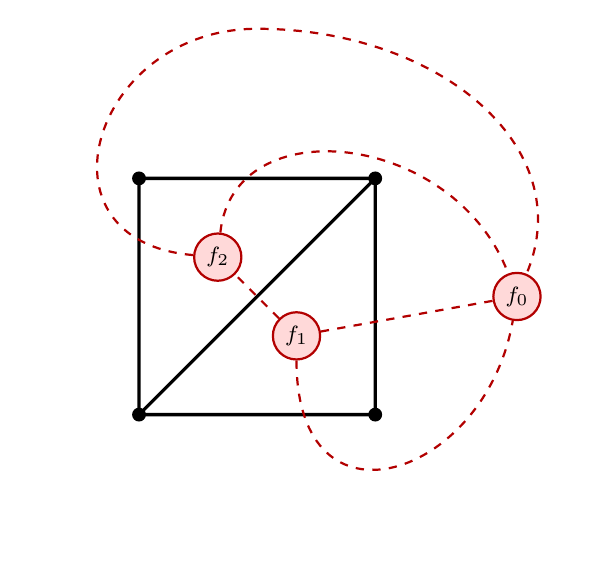
\begin{tikzpicture}[
  vertex/.style={circle, fill, inner sep=0pt, minimum size=5pt},
  dual/.style={circle, draw=red!70!black, fill=red!15, thick, inner sep=0pt, minimum size=6mm, font=\footnotesize},
  dualedge/.style={thick, red!70!black, dashed},
]
  \coordinate (a) at (0,0);
  \coordinate (b) at (3,0);
  \coordinate (c) at (3,3);
  \coordinate (d) at (0,3);
  \draw[very thick] (a) -- (b) -- (c) -- (d) -- cycle (a) -- (c);
  \foreach \p in {a,b,c,d} \node[vertex] at (\p) {};
  % The dual vertices of the two triangles sit at their centroids; f0 stands for the outer face.
  \node[dual] (f1) at (2,1) {$f_1$};
  \node[dual] (f2) at (1,2) {$f_2$};
  \node[dual] (o) at (4.8,1.5) {$f_0$};
  \draw[dualedge] (f1) -- (f2);
  \draw[dualedge] (f1) -- (o);
  % The other four dual edges leave through the bottom, top, and left sides and loop round to f0 without crossing
  \draw[dualedge] (f1) .. controls (2,-1.6) and (4.4,-0.8) .. (o);
  \draw[dualedge] (f2) .. controls (1.2,3.9) and (4,3.6) .. (o);
  \draw[dualedge] (f2) .. controls (-1.4,2.2) and (-0.6,4.9) .. (1.5,4.9) .. controls (3.8,4.9) and (5.6,3.4) .. (o);
\end{tikzpicture}
